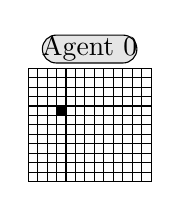
\begin{tikzpicture}[scale=0.12]
        \filldraw[fill=gray!20, rounded corners=5pt] (1.5,15.5) rectangle ++(10,-2.95) node[midway,align=center]{Agent 0};
        \foreach \x in {0,...,12}{
            \foreach \y in {0,...,11}{
                \draw (\x,\y) rectangle ++(1,1);
            }
        }
        \fill[black] (3,7) rectangle ++(1, 1);
    \end{tikzpicture} 
    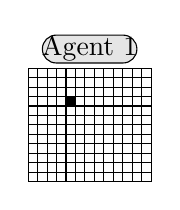
\begin{tikzpicture}[scale=0.12]
        \filldraw[fill=gray!20, rounded corners=5pt] (1.5,15.5) rectangle ++(10,-2.95) node[midway,align=center]{Agent 1};
        \foreach \x in {0,...,12}{
            \foreach \y in {0,...,11}{
                \draw (\x,\y) rectangle ++(1,1);
            }
        }
        \fill[black] (4,8) rectangle ++(1, 1);
    \end{tikzpicture}
    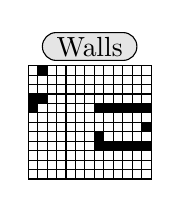
\begin{tikzpicture}[scale=0.12]
        \filldraw[fill=gray!20, rounded corners=5pt] (1.5,15.5) rectangle ++(10,-2.95) node[midway,align=center]{Walls};
        \foreach \x in {0,...,12}{
            \foreach \y in {0,...,11}{
                \draw (\x,\y) rectangle ++(1,1);
            }
        }
        \fill[black] (0,7) rectangle ++(1, 1);
        \fill[black] (0,8) rectangle ++(1, 1);
        \fill[black] (1,8) rectangle ++(1, 1);
        \fill[black] (1,11) rectangle ++(1, 1);

        \foreach \x in {7,...,12}{
            \fill[black] (\x,7) rectangle ++(1, 1);
        }

        \foreach \x in {7,...,12}{
            \fill[black] (\x,3) rectangle ++(1, 1);
        }
        \fill[black] (7,4) rectangle ++(1, 1);
        \fill[black] (12,5) rectangle ++(1, 1);
    \end{tikzpicture}
    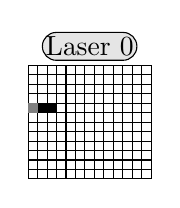
\begin{tikzpicture}[scale=0.12]
        \filldraw[fill=gray!20, rounded corners=5pt] (1.5,15.5) rectangle ++(10,-2.95) node[midway,align=center]{Laser 0};
        \foreach \x in {0,...,12}{
            \foreach \y in {0,...,11}{
                \draw (\x,\y) rectangle ++(1,1);
            }
        }
        \fill[gray] (0,7) rectangle ++(1, 1);
        \fill[black] (1,7) rectangle ++(1, 1);
        \fill[black] (2,7) rectangle ++(1, 1);
    \end{tikzpicture}
    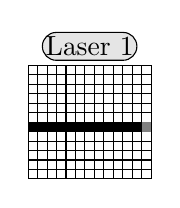
\begin{tikzpicture}[scale=0.12]
        \filldraw[fill=gray!20, rounded corners=5pt] (1.5,15.5) rectangle ++(10,-2.95) node[midway,align=center]{Laser 1};
        \foreach \x in {0,...,12}{
            \foreach \y in {0,...,11}{
                \draw (\x,\y) rectangle ++(1,1);
            }
        }
        \foreach \x in {0,...,11}{
            \fill[black] (\x,5) rectangle ++(1, 1);
        }
        \fill[gray] (12,5) rectangle ++(1, 1);
    \end{tikzpicture}
    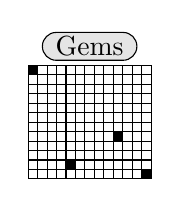
\begin{tikzpicture}[scale=0.12]
        \filldraw[fill=gray!20, rounded corners=5pt] (1.5,15.5) rectangle ++(10,-2.95) node[midway,align=center]{Gems};
        \foreach \x in {0,...,12}{
            \foreach \y in {0,...,11}{
                \draw (\x,\y) rectangle ++(1,1);
            }
        }
        \fill[black] (0,11) rectangle ++(1, 1);
        \fill[black] (12,0) rectangle ++(1, 1);
        \fill[black] (4,1) rectangle ++(1, 1);
        \fill[black] (9,4) rectangle ++(1, 1);
    \end{tikzpicture}
    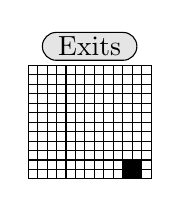
\begin{tikzpicture}[scale=0.12]
        \filldraw[fill=gray!20, rounded corners=5pt] (1.5,15.5) rectangle ++(10,-2.95) node[midway,align=center]{Exits};
        \foreach \x in {0,...,12}{
            \foreach \y in {0,...,11}{
                \draw (\x,\y) rectangle ++(1,1);
            }
        }
        \foreach \x in {10,...,11}{
            \foreach \y in {0,...,1}{
                \fill[black] (\x,\y) rectangle ++(1, 1);
            }
        }
    \end{tikzpicture}
